%!TEX program = xelatex
\documentclass{template/document}
%%%%%%%%%%%%%%%%%%%%%%%%%%%%%%%%%%%%%%%%%%%%%%%%%%%%%%%%%%%%%%%%%%%%%%%%%%%%%%%%
% Fonts
%%%%%%%%%%%%%%%%%%%%%%%%%%%%%%%%%%%%%%%%%%%%%%%%%%%%%%%%%%%%%%%%%%%%%%%%%%%%%%%%
\newcommand\SectionFontStyle{\fontspec[
	Path=./template/fonts/Open_Sans/,
	Extension=.ttf,
	UprightFont=*-Regular,
	BoldFont=*-Bold,
	ItalicFont=*-Italic,
	BoldItalicFont=*-BoldItalic
	]{OpenSans}
}

% Better monoscript font
\setmonofont{DejaVu Sans Mono}

\pgfplotsset{compat=1.7}
\linespread{1.3}

\setkomafont{chapter}{\huge\SectionFontStyle}           % Chapter
\setkomafont{sectioning}{\SectionFontStyle}             % Section
\setkomafont{pagenumber}{\bfseries\SectionFontStyle}    % Pagenumber
\setkomafont{pagehead}{\small\sffamily}                 % Heading
\setkomafont{descriptionlabel}{\itshape}                % Heading

% fix font-size of urls in bibliography
\AtBeginBibliography{\def\UrlFont{\scriptsize\tt}}

% Some shortcuts for fontawesome
\def\oneStar{\faStar}
\def\twoStars{\faStar\faStar}
\def\threeStars{\faStar\faStar\faStar}

%%%%%%%%%%%%%%%%%%%%%%%%%%%%%%%%%%%%%%%%%%%%%%%%%%%%%%%%%%%%%%%%%%%%%%%%%%%%%%%%
% Encoding of TOC (and hyperlinks in general)
%%%%%%%%%%%%%%%%%%%%%%%%%%%%%%%%%%%%%%%%%%%%%%%%%%%%%%%%%%%%%%%%%%%%%%%%%%%%%%%%
\hypersetup{pdfencoding=auto}

%%%%%%%%%%%%%%%%%%%%%%%%%%%%%%%%%%%%%%%%%%%%%%%%%%%%%%%%%%%%%%%%%%%%%%%%%%%%%%%%
% Colors
%%%%%%%%%%%%%%%%%%%%%%%%%%%%%%%%%%%%%%%%%%%%%%%%%%%%%%%%%%%%%%%%%%%%%%%%%%%%%%%%
% \definecolor    color-syntax
% \colorlet       xcolor-syntax

\definecolor{titlepagecolor}{HTML}{0D3F6E}
\definecolor{titlepagefontcolor}{RGB}{255,255,255}

\definecolor{sectioncolor}{RGB}{0, 0, 0}
\colorlet{chaptercolor}{titlepagefontcolor}

\colorlet{tablesubheadcolor}{gray!30}
\colorlet{tableheadcolor}{gray!25}
\colorlet{tableblackheadcolor}{black!100}
\colorlet{tablerowcolor}{gray!10.0}

\colorlet{listingbackground}{gray!10.0}
\colorlet{stringcolor}{green!40!black!100}
\colorlet{commentcolor}{green!40!black!100}


\addtokomafont{chapter}{\color{chaptercolor}}           % Chapter Font
\addtokomafont{sectioning}{\color{sectioncolor}}        % Section Font


%%%%%%%%%%%%%%%%%%%%%%%%%%%%%%%%%%%%%%%%%%%%%%%%%%%%%%%%%%%%%%%%%%%%%%%%%%%%%%%%
% Page Dimensions
%%%%%%%%%%%%%%%%%%%%%%%%%%%%%%%%%%%%%%%%%%%%%%%%%%%%%%%%%%%%%%%%%%%%%%%%%%%%%%%%
\geometry{
 a4paper,
 total={210mm,297mm},
 left=20mm,
 right=20mm,
 top=20mm,
 bottom=20mm,
 }
 
%%%%%%%%%%%%%%%%%%%%%%%%%%%%%%%%%%%%%%%%%%%%%%%%%%%%%%%%%%%%%%%%%%%%%%%%%%%%%%%%
% Page Heading
%%%%%%%%%%%%%%%%%%%%%%%%%%%%%%%%%%%%%%%%%%%%%%%%%%%%%%%%%%%%%%%%%%%%%%%%%%%%%%%%
\renewcommand*{\raggedsection}{\raggedright} % Titelzeile linksbuendig, haengend

\pagestyle{scrheadings} % Seite mit Headern
\clearscrheadings
\clearscrplain
	\ohead{\pagemark}
	\ihead{\headmark}
		\automark[section]{chapter}
		\setheadsepline{.4pt}[\color{black}]
\setheadwidth[0pt]{text}
\setfootwidth[0pt]{text}


%%%%%%%%%%%%%%%%%%%%%%%%%%%%%%%%%%%%%%%%%%%%%%%%%%%%%%%%%%%%%%%%%%%%%%%%%%%%%%%%
% Chapter
%%%%%%%%%%%%%%%%%%%%%%%%%%%%%%%%%%%%%%%%%%%%%%%%%%%%%%%%%%%%%%%%%%%%%%%%%%%%%%%%
\titleformat{\chapter}[block]%
		{\usekomafont{chapter}\Large\color{chaptercolor}\bfseries % Chaptertitle Format
		\tikz[overlay]\path [fill=titlepagecolor](50mm,240mm)circle[x radius=290mm, y radius=250mm];} % Backgroundshape
		{\normalfont\usekomafont{chapter}\large \chaptertitlename \hspace{0.1em} \thechapter} % "Chapter XY" formatting
		{0.8em} % Space betweend "Chapter XY" and Chaptername
		{} % Before
		[\vspace{5mm}] % After


%%%%%%%%%%%%%%%%%%%%%%%%%%%%%%%%%%%%%%%%%%%%%%%%%%%%%%%%%%%%%%%%%%%%%%%%%%%%%%%%
% Footnotes
%%%%%%%%%%%%%%%%%%%%%%%%%%%%%%%%%%%%%%%%%%%%%%%%%%%%%%%%%%%%%%%%%%%%%%%%%%%%%%%%
\deffootnote{1.5em}{1em}{\makebox[1.5em][l]{\thefootnotemark}}
\addtolength{\skip\footins}{\baselineskip}      % Abstand Text <-> Fussnote
\setlength{\dimen\footins}{10\baselineskip}     % Beschraenkt den Platz von
												% Fussnoten auf 10 Zeilen
\interfootnotelinepenalty=10000                 % Verhindert das Fortsetzen von
												% Fussnoten auf der
												% gegenüberligenden Seite


%%%%%%%%%%%%%%%%%%%%%%%%%%%%%%%%%%%%%%%%%%%%%%%%%%%%%%%%%%%%%%%%%%%%%%%%%%%%%%%%
% Table of Contents/Figures/Tables
%%%%%%%%%%%%%%%%%%%%%%%%%%%%%%%%%%%%%%%%%%%%%%%%%%%%%%%%%%%%%%%%%%%%%%%%%%%%%%%%
\setcounter{secnumdepth}{3}       % Abbildungsnummerierung mit groesserer Tiefe
\setcounter{tocdepth}{2}          % Inhaltsverzeichnis mit groesserer Tiefe

\usetocstyle{allwithdot}
% sans serif fonts for all levels
\settocfeature[toc][0]{entryhook}{\sffamily}
\settocfeature[toc][1]{entryhook}{\sffamily}
\settocfeature[toc][2]{entryhook}{\sffamily}
\settocfeature[toc][3]{entryhook}{\sffamily}

% Figure and Table Directory one level deeper in hierarchy:
\KOMAoption{listof}{leveldown}

%%%%%%%%%%%%%%%%%%%%%%%%%%%%%%%%%%%%%%%%%%%%%%%%%%%%%%%%%%%%%%%%%%%%%%%%%%%%%%%%
% Bibliography
%%%%%%%%%%%%%%%%%%%%%%%%%%%%%%%%%%%%%%%%%%%%%%%%%%%%%%%%%%%%%%%%%%%%%%%%%%%%%%%%
%\bibliographystyle {alpha}

% Redefine the bibliography chapter title from "chapter*{...}" to "chapter{...}":
%\renewcommand{\bibsection}{\chapter{\bibname}}
\defbibheading{references}[\refname]{\chapter{#1}}


%%%%%%%%%%%%%%%%%%%%%%%%%%%%%%%%%%%%%%%%%%%%%%%%%%%%%%%%%%%%%%%%%%%%%%%%%%%%%%%%
% Glossary
%%%%%%%%%%%%%%%%%%%%%%%%%%%%%%%%%%%%%%%%%%%%%%%%%%%%%%%%%%%%%%%%%%%%%%%%%%%%%%%%
\setglossarysection{chapter}


%%%%%%%%%%%%%%%%%%%%%%%%%%%%%%%%%%%%%%%%%%%%%%%%%%%%%%%%%%%%%%%%%%%%%%%%%%%%%%%%
% enumitem
%%%%%%%%%%%%%%%%%%%%%%%%%%%%%%%%%%%%%%%%%%%%%%%%%%%%%%%%%%%%%%%%%%%%%%%%%%%%%%%%
\setlist{noitemsep}
\setlist[itemize]{
    nolistsep,
    noitemsep,
    before*={\mbox{}\vspace{-\baselineskip}}
}
\setlist[itemize,2] {
    before*={\mbox{}\vspace{\baselineskip}}
}


%%%%%%%%%%%%%%%%%%%%%%%%%%%%%%%%%%%%%%%%%%%%%%%%%%%%%%%%%%%%%%%%%%%%%%%%%%%%%%%%
% Code Listings
%%%%%%%%%%%%%%%%%%%%%%%%%%%%%%%%%%%%%%%%%%%%%%%%%%%%%%%%%%%%%%%%%%%%%%%%%%%%%%%%
\lstset{
	basicstyle=\small\ttfamily, % Standardschrift
	numbers=left,               % Ort der Zeilennummern
	numberstyle=\tiny,          % Stil der Zeilennummern
	numbersep=5pt,              % Abstand der Nummern zum Text
	tabsize=2,                  % Groesse von Tabs
	extendedchars=true,         %
	breaklines=true,            % Zeilen werden Umgebrochen
	backgroundcolor=\color{listingbackground},
	stringstyle=\color{stringcolor}, % Farbe der String
	commentstyle=\color{commentcolor}, % Farbe der String
	showspaces=false,           % Leerzeichen anzeigen ?
	showtabs=false,             % Tabs anzeigen ?
	showstringspaces=false,      % Leerzeichen in Strings anzeigen ?
	language=Java,
	captionpos=b,
	abovecaptionskip=5mm,
	frame=tb,
	framerule=0pt,
	framesep=0pt,
	framexleftmargin=5pt,
	framexrightmargin=5pt,
	framextopmargin=5pt,
	framexbottommargin=5pt
}

\renewcommand{\lstlistlistingname}{Quelltexte}
\renewcommand{\lstlistingname}{Quelltext}

\definecolor{lightgray}{rgb}{.9,.9,.9}
\definecolor{darkgray}{rgb}{.4,.4,.4}
\definecolor{purple}{rgb}{0.65, 0.12, 0.82}

\lstdefinelanguage{JavaScript}{
	keywords={typeof, new, true, false, catch, function, return, null, catch, switch, var, if, in, while, do, else, case, break},
	keywordstyle=\color{blue}\bfseries,
	ndkeywords={class, export, boolean, throw, implements, import, this},
	ndkeywordstyle=\color{darkgray}\bfseries,
	identifierstyle=\color{black},
	sensitive=false,
	comment=[l]{//},
	morecomment=[s]{/*}{*/},
	commentstyle=\color{purple}\ttfamily,
	stringstyle=\color{red}\ttfamily,
	morestring=[b]',
	morestring=[b]"
}

\lstset{
	language=JavaScript,
	backgroundcolor=\color{lightgray},
	extendedchars=true,
	basicstyle=\footnotesize\ttfamily,
	showstringspaces=false,
	showspaces=false,
	numbers=left,
	numberstyle=\footnotesize,
	numbersep=9pt,
	tabsize=2,
	breaklines=true,
	showtabs=false,
	captionpos=b
}

\lstdefinelanguage{CSharp}{
 	morekeywords = {abstract,event,new,struct,as,explicit,%
    null,switch,base,extern,object,this,bool,false,%
    operator,throw,break,finally,out,true,byte,fixed,%
    override,try,case,float,params,typeof,catch,for,%
    private,uint,char,foreach,protected,ulong,checked,%
    goto,public,unchecked,class,if,readonly,unsafe,%
    const,implicit,ref,ushort,continue,in,return,using,%
    decimal,int,sbyte,virtual,default,interface,sealed,%
    volatile,delegate,internal,short,void,do,is,sizeof,%
    while,double,lock,stackalloc,else,long,static,%
    enum,namespace,string,partial},
  morecomment = [l]{//},
  morecomment = [l]{///},
  morecomment = [s]{/*}{*/},
  morestring=[b]",
  sensitive = true
}
\newcommand{\lstsetcsharp}{
 	\lstset{language=CSharp,
        breaklines=true,
        commentstyle=\sffamily,
        basicstyle=\sffamily,
        keywordstyle=\bfseries,
        stringstyle=\ttfamily,
        showstringspaces=false,
        frame=single,
        tabsize=2,
        linewidth=\textwidth,captionpos=b
        numbers=left, stepnumber=5, numbersep=10pt
 	}
}

\newcommand{\lstsethtml}{
 	\lstset{language=HTML,
        breaklines=true,
        commentstyle=\textit,
        keywordstyle=\bfseries,
        basicstyle=\ttfamily,
        stringstyle=\ttfamily,
        showstringspaces=false,
        frame=single,
        tabsize=2
        %%linewidth=\textwidth,captionpos=b
        %numbers=left, stepnumber=5, numbersep=10pt
 	}
}

\newcommand{\lstsetxml}{
 	\lstset{language=XML,
        breaklines=true,
        commentstyle=\sffamily,
        keywordstyle=\bfseries,
        basicstyle=\sffamily,
        showstringspaces=false,
        stringstyle=\ttfamily,
        frame=single,
        tabsize=2,
        literate=
        %linewidth=\textwidth,captionpos=b
        %numbers=left, stepnumber=5, numbersep=10pt
 	}
}


%%%%%%%%%%%%%%%%%%%%%%%%%%%%%%%%%%%%%%%%%%%%%%%%%%%%%%%%%%%%%%%%%%%%%%%%%%%%%%%%
% Tables
%%%%%%%%%%%%%%%%%%%%%%%%%%%%%%%%%%%%%%%%%%%%%%%%%%%%%%%%%%%%%%%%%%%%%%%%%%%%%%%%
%
% http://www.matthiaspospiech.de/latex/vorlagen/
%

%%% -| Neue Spaltendefinitionen 'columntypes' |--
%
% Belegte Spaltentypen:
% l - links
% c - zentriert
% r - rechts
% p,m,b  - oben, mittig, unten
% X - tabularx Auto-Spalte

% um Tabellenspalten mit Flattersatz zu setzen, muss \\ vor
% (z.B.) \raggedright geschuetzt werden:
\newcommand{\PreserveBackslash}[1]{\let\temp=\\#1\let\\=\temp}


% Spalten mit Flattersatz und definierte Breite:
% m{} -> mittig
% p{} -> oben
% b{} -> unten
%
% Linksbuendig:
\newcolumntype{v}[1]{>{\PreserveBackslash\RaggedRight\hspace{0pt}}p{#1}}
\newcolumntype{M}[1]{>{\PreserveBackslash\RaggedRight\hspace{0pt}}m{#1}}
% % Rechtsbuendig :
% \newcolumntype{R}[1]{>{\PreserveBackslash\RaggedLeft\hspace{0pt}}m{#1}}
% \newcolumntype{S}[1]{>{\PreserveBackslash\RaggedLeft\hspace{0pt}}p{#1}}
% % Zentriert :
% \newcolumntype{Z}[1]{>{\PreserveBackslash\Centering\hspace{0pt}}m{#1}}
% \newcolumntype{A}[1]{>{\PreserveBackslash\Centering\hspace{0pt}}p{#1}}

\newcolumntype{Y}{>{\PreserveBackslash\RaggedLeft\hspace{0pt}}X}

% Tabellenspaltentyp fuer den Kopf: (Farbe + Ausrichtung)
\newcolumntype{H}[1]{>{\columncolor{tableheadcolor}}l}



%%% ---|Layout der Tabellen |-------------------

% Neue Umgebung fuer Tabellen:

\newenvironment{Tabelle}[2][c]{%
	\tablestylecommon
	\begin{longtable}[#1]{#2}
	}
	{\end{longtable}%
	\tablerestoresettings
}


% Groesse der Schrift in Tabellen
\newcommand{\tablefontsize}{ \footnotesize}
\newcommand{\tableheadfontsize}{\footnotesize}

% Layout der Tabelle: Ausrichtung, Schrift, Zeilenabstand
\newcommand\tablestylecommon{%
	\renewcommand{\arraystretch}{1.4} % Groessere Abstaende zwischen Zeilen
	\normalfont\normalsize            %
	\sffamily\tablefontsize           % Serifenlose und kleine Schrift
	\centering%                       % Tabelle zentrieren
}

\newcommand{\tablestyle}{
	\tablestylecommon
	%\tablealtcolored
}

% Ruecksetzten der Aenderungen
\newcommand\tablerestoresettings{%
	\renewcommand{\arraystretch}{1}% Abstaende wieder zuruecksetzen
	\normalsize\rmfamily % Schrift wieder zuruecksetzen
}

% Tabellenkopf: Serifenlos+fett+schraeg+Schriftfarbe
\renewcommand\tablehead{%
	\tableheadfontsize%
	\sffamily\bfseries%
	\slshape
	%\color{white}
}

\newcommand\tablesubheadfont{%
	\tableheadfontsize%
	\sffamily\bfseries%
	\slshape
	%\color{white}
}


\newcommand\tableheadcolor{%
	%\rowcolor{tablesubheadcolor}
	%\rowcolor{tableblackheadcolor}
	\rowcolor{tableheadcolor}%
}

\newcommand\tablesubheadcolor{%
	%\rowcolor{tablesubheadcolor}
	%\rowcolor{tableblackheadcolor}
}


\newcommand{\tableend}{\arrayrulecolor{black}\hline}

% Tabellenkopf (1=Spaltentyp, 2=Text)
% \newcommand{\tablehead}[2]{
%   \multicolumn{1}{#1@{}}{%
%     \raisebox{.1mm}{% Ausrichtung der Beschriftung
%       #2%
%     }\rule{0pt}{4mm}}% unsichtbare Linie, die die Kopfzeile hoeher macht
% }


\newcommand{\tablesubhead}[2]{%
	\multicolumn{#1}{>{\columncolor{tablesubheadcolor}}l}{\tablesubheadfont #2}%
}

% Tabellenbody (=Inhalt)
\newcommand\tablebody{%
\tablefontsize\sffamily\upshape%
}

\newcommand\tableheadshaded{%
	\rowcolor{tableheadcolor}%
}
\newcommand\tablealtcolored{%
	\rowcolors{1}{tablerowcolor}{white!100}%
}
%%% --------------------------------------------


\newcommand\documentTitle{Domainanalyse Projekt VoluntaryO}
\newcommand\documentAuthorA{Dominik Freier}
\newcommand\documentAuthorB{Nhat-Nam Le}
\newcommand\documentAuthorC{Philipp Meier}
\newcommand\documentAuthorD{Robin Bader}
\newcommand\documentSubject{Software Engineering 2 - Projekt}

\makeindex

\begin{document}
 
    \newcommand\documentTerm{Frühjahrssemester 2014}
\newcommand\documentSchool{Hochschule für Technik Rapperswil}
\newcommand\documentProfessor{Prof. Dr.  Luc Bläser}
\newcommand\documentCrossReader{tbd}

\hypersetup{
    pdfauthor={\documentAuthorA, \documentAuthorB, \documentAuthorC, \documentAuthorD},
    pdftitle={\documentTitle},
    pdfsubject={\documentSubject}
}

\begin{titlepage}
    % Page Settings:
    \newgeometry{top=110mm,right=30mm,bottom=20mm,left=30mm}
    \backgroundsetup{scale=1,angle=0,opacity=1,contents={
        \begin{tikzpicture}[remember picture,overlay]
            \path [fill=titlepagecolor]
            (0,-175mm)circle[x radius=290mm, y radius=250mm];
            \node [anchor=south west] (image) at (-0.5\paperwidth+8mm,0.5\paperheight-39mm) {
\includegraphics[height=25mm]{template/images/hsrlogo.png}};
            \node [anchor=south east] (image) at (0.4\paperwidth+8mm,0.5\paperheight-39mm) {
\includegraphics[height=25mm]{template/images/voluntaryo_logo.png}};
        \end{tikzpicture}}
    }

    % Apply Page settings:
    \thispagestyle{empty}
    \BgThispage

    % Content:
    \sffamily\color{titlepagefontcolor}
    \begin{center}
        \Large
        \documentSubject\\[5mm]

        \Huge\bfseries
        \documentTitle\\[15mm]

        \large\normalfont\sffamily
        \documentSchool\\[1mm]
        \documentTerm\\[15mm]

        \vfill
        \normalsize\normalfont\sffamily
        Erstellt: \today, \currenttime\\[10mm]
    \end{center}


    \begin{multicols}{2}

        \begin{tabularx}{\textwidth}{X}
            \bfseries \documentAuthorA\tabularnewline
            \bfseries \documentAuthorB\tabularnewline
            \bfseries \documentAuthorC\tabularnewline
            \bfseries \documentAuthorD\tabularnewline
        \end{tabularx}

        \begin{tabularx}{\textwidth}{l X}
            \bfseries Betreuer & \documentProfessor\tabularnewline
            \bfseries Gegenleser & \documentCrossReader\tabularnewline
        \end{tabularx}
    \end{multicols}

\end{titlepage}

\restoregeometry


    \tableofcontents
    \newpage

    \section*{Änderungshistorie}
    \begin{table}[H]
        \tablestyle
        \tablealtcolored
        \begin{tabularx}{\textwidth}{l l X r}
        \tableheadcolor
            \tablehead Version & 
            \tablehead Datum & 
            \tablehead Änderung & 
            \tablehead Person \\  
        \tablebody
            v1.0 & 11.03.2014 & Initialisierung & nle \tabularnewline
            v1.1 & 11.03.2014 & Systemoperationen und Systemsequenzdiagramme & r1bader \tabularnewline
            v1.2 & 12.03.2014 & Domainmodell & dfreier, p1meier \tabularnewline
            v1.3 & 25.03.2014 & Review E1 Verbesserungen & dfreier \tabularnewline
        \tableend
        \end{tabularx} 
    \end{table}
    \newpage

    \chapter{Einführung}
    %!TEX root = ../../domainanalyse.tex
\chapter{Domain Modell}
	\section{Domain Model}
		\begin{figure}[ht]
		    \center
			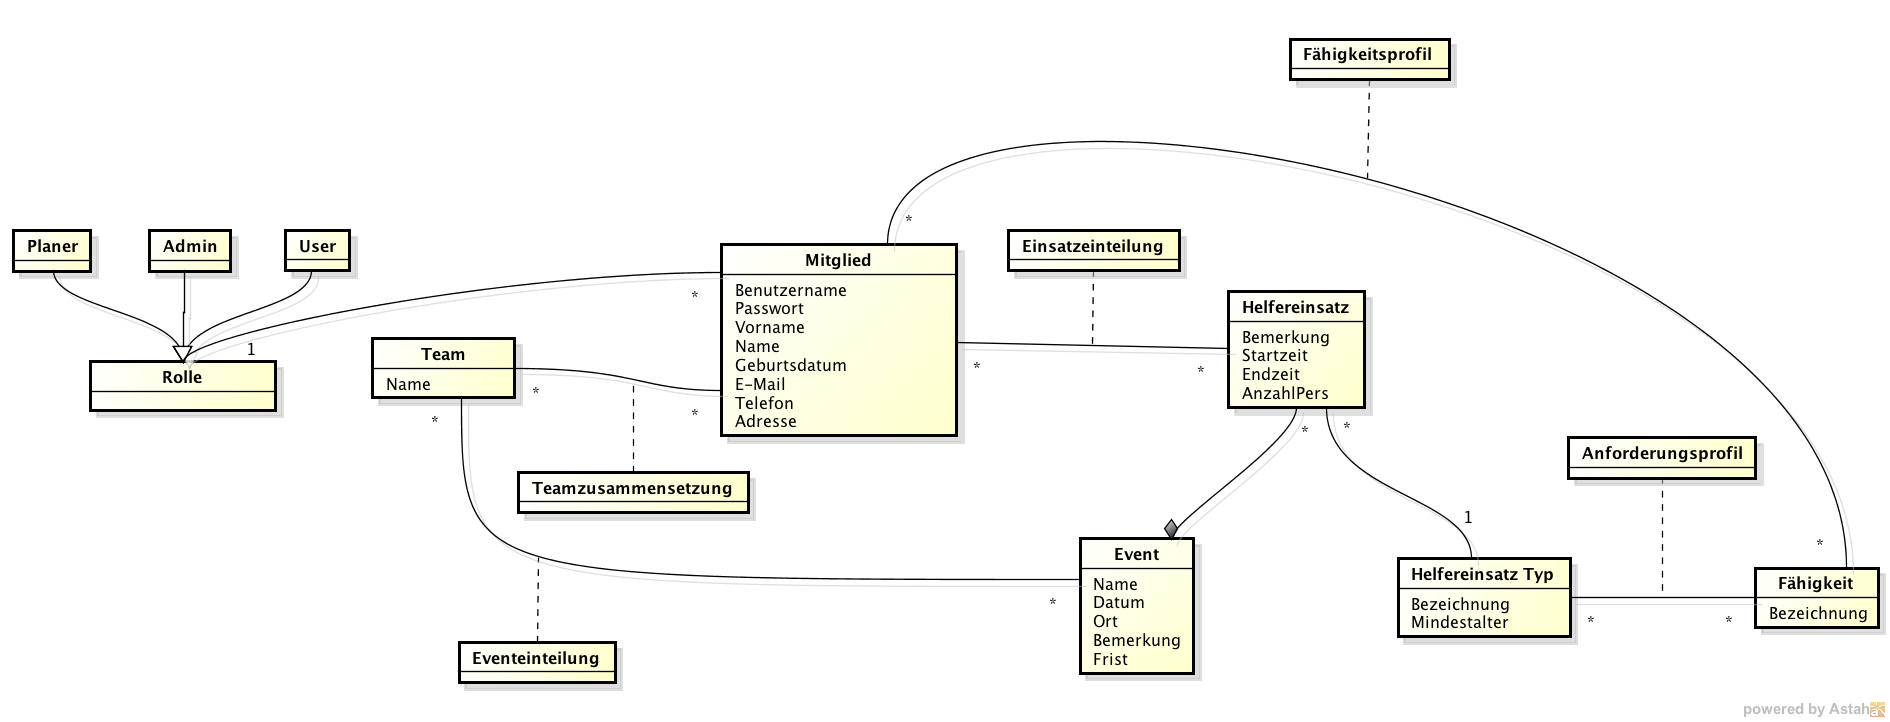
\includegraphics[width=\textwidth]{content/domainanalyse/images/Domainmodell_mit_Assoziationen.png}
		    \caption{Domainmodell mit Assoziationen}
		\end{figure}

	\section{Klassenspezifikation}
	\subsection{Event}
	Ein \underline{Event} stellt einen Anlass bzw. einen Spieltag dar, für den es Helfer braucht, um gewisse Aufgaben zu erledigen. Es gibt vor, welche Aufgaben (\underline{Helfereinsätze}) verteilt werden müssen und welche \underline{\underline{Mitglieder}} dazu in frage kommen. Letzteres geschieht über die Zuordnung von \underline{Teams}.

	\subsubsection*{Attribute}
    \begin{table}[H]
        \tablestyle
        \tablealtcolored
        \begin{tabularx}{\textwidth}{l l X}
        \tableheadcolor
            \tablehead Attribut & 
            \tablehead Typ & 
            \tablehead Beschreibung \tabularnewline  
        \tablebody
			Name      & String & Name des Events \tabularnewline                                                  
			Datum     & Date   & Durchführungsdatum \tabularnewline                                               
			Ort       & String & Freie Ortsangabe, ohne Adressformat \tabularnewline                              
			Bemerkung & String & Optionale Bemerkung zum Event. Kann längeren Text beinhalten. \tabularnewline    
			Frist     & Date   & Datum, ab welchem keine An- und Abmeldungen mehr zugelassen sind. \tabularnewline 
        \tableend
        \end{tabularx} 
    \end{table}

    \subsubsection*{Relationen}
    \begin{table}[H]
        \tablestyle
        \tablealtcolored
        \begin{tabularx}{\textwidth}{l l l X}
        \tableheadcolor
            \tablehead Nr & 
            \tablehead Klasse & 
            \tablehead Multiplizität & 
            \tablehead Beschreibung \tabularnewline  
        \tablebody
			1 & \underline{Helfereinsatz} & 1:n & Legt fest, welche Helfereinsätze zum Event gehören. \tabularnewline 
			2 & \underline{Team} & n:m & Dient dazu, Mitglieder für Helfereinsätze freizuschalten. Pro Event können mehrere Teams zuständig sein. \tabularnewline 
        \tableend
        \end{tabularx} 
    \end{table}

    \subsection{Mitglied}
    Ein \underline{Mitglied} stellt sowohl ein Mitglied des Vereins, als auch einen Benutzer des Systems dar. \underline{Mitglieder} werden für \underline{Helfereinsätze} eingeteilt.

    \subsubsection*{Attribute}
    \begin{table}[H]
        \tablestyle
        \tablealtcolored
        \begin{tabularx}{\textwidth}{l l X}
        \tableheadcolor
            \tablehead Attribut & 
            \tablehead Typ & 
            \tablehead Beschreibung \tabularnewline  
        \tablebody
			Benutzername & String  & Anmeldename für den Benutzer. \tabularnewline  
			Passwort     & String  & Zum Benutzernamen gehöriges Passwort für Anmeldung. \tabularnewline  
			Vorname      & String  & Vorname des \underline{Mitglieds} \tabularnewline  
			Name         & String  & Nachname des \underline{Mitglieds} \tabularnewline  
			Geburtsdatum & Date    & Geburtsdatum des \underline{Mitglieds} \tabularnewline  
			E-Mail       & String  & E-Mail Adresse des \underline{Mitglieds} \tabularnewline  
			Telefon      & String  & Optional: Telefonnummer des \underline{Mitglieds} \tabularnewline  
			Adresse      & Address & Wohnadresse/Anschrift des \underline{Mitglieds}. \tabularnewline  
        \tableend
        \end{tabularx} 
    \end{table}

    \subsubsection*{Relationen}
    \begin{table}[H]
        \tablestyle
        \tablealtcolored
        \begin{tabularx}{\textwidth}{l l l X}
        \tableheadcolor
            \tablehead Nr & 
            \tablehead Klasse & 
            \tablehead Multiplizität & 
            \tablehead Beschreibung \tabularnewline  
        \tablebody
			3 & \underline{Team}          & n:m & Beschreibt, welche \underline{Mitglieder} in welchen \underline{Teams} sind. Ein Mitglied kann auch zu mehreren \underline{Teams} gehören. \tabularnewline
			4 & \underline{Rolle}         & n:1 & Zuweisung von Rolle an \underline{Mitglieder}. \tabularnewline
			5 & \underline{Fähigkeit}     & n:m & Legt fest, welche Fähigkeiten ein \underline{Mitglied} besitzt. \tabularnewline
			6 & \underline{Helfereinsatz} & n:m & Zuordnung von Helfereinsätzen und \underline{Mitglieder}n. Damit die Verbindung zulässig ist, müssen \underline{Anforderungsprofil} und \underline{Fähigkeitsprofil} übereinstimmen. \tabularnewline
        \tableend
        \end{tabularx} 
    \end{table}

    \subsection{Team}
	Stellt eine Mannschaft des Vereins dar und kann einem \underline{Event} zugeordnet werden. Die dazugehörigen \underline{Mitglieder} werden somit für die \underline{Helfereinsätze} des \underline{Events} freigeschaltet.

    \subsubsection*{Attribute}
    \begin{table}[H]
        \tablestyle
        \tablealtcolored
        \begin{tabularx}{\textwidth}{l l X}
        \tableheadcolor
            \tablehead Attribut & 
            \tablehead Typ & 
            \tablehead Beschreibung \tabularnewline  
        \tablebody
			Name & String  & Name der Mannschaft. \tabularnewline 
        \tableend
        \end{tabularx} 
    \end{table}

    \subsubsection*{Relationen}
    \begin{table}[H]
        \tablestyle
        \tablealtcolored
        \begin{tabularx}{\textwidth}{l l l X}
        \tableheadcolor
            \tablehead Nr & 
            \tablehead Klasse & 
            \tablehead Multiplizität & 
            \tablehead Beschreibung \tabularnewline  
        \tablebody
			7 & \underline{Mitglied} & m:n & Inversion \#3 \tabularnewline  
			8 & \underline{Event}    & m:n & Inversion \#2 \tabularnewline  
        \tableend
        \end{tabularx} 
    \end{table}

    \subsection{Helfereinsatz Typ}
	Diese Klasse dient als Vorlage für \underline{Helfereinsätze}. Sie beschreibt eine gewisse Tätigkeit und definiert die Anforderungen (\underline{Fähigkeiten}), welche ein \underline{Mitglied} erfüllen muss, um sich für einen \underline{Helfereinsatz} dieses Typs anmelden zu können.

    \subsubsection*{Attribute}
    \begin{table}[H]
        \tablestyle
        \tablealtcolored
        \begin{tabularx}{\textwidth}{l l X}
        \tableheadcolor
            \tablehead Attribut & 
            \tablehead Typ & 
            \tablehead Beschreibung \tabularnewline  
        \tablebody
			Bezeichnung  & String  & Titel/Bezeichung des Typs \tabularnewline  
			Mindestalter & Integer & Mindestalter, welches ein \underline{Mitglied} haben muss, um sich für einen \underline{Helfereinsatz} dieses Typs anmelden zu können. \tabularnewline  
        \tableend
        \end{tabularx} 
    \end{table}

    \subsubsection*{Relationen}
    \begin{table}[H]
        \tablestyle
        \tablealtcolored
        \begin{tabularx}{\textwidth}{l l l X}
        \tableheadcolor
            \tablehead Nr & 
            \tablehead Klasse & 
            \tablehead Multiplizität & 
            \tablehead Beschreibung \tabularnewline  
        \tablebody
			9  & \underline{Helfereinsatz} & 1:n & Inversion von \#15 \tabularnewline
			10 & \underline{Fähigkeit}     & n:m & Definiert vorausgesetzte \underline{Fähigkeiten} für Typ \tabularnewline
        \tableend
        \end{tabularx} 
    \end{table}

    \subsection{Fähigkeit}
	Fähigkeiten/Kompetenzen, die \underline{Mitglieder} haben können, um sich dadurch für bestimmte \underline{Helfereinsätze} zu qualifizieren.

    \subsubsection*{Attribute}
    \begin{table}[H]
        \tablestyle
        \tablealtcolored
        \begin{tabularx}{\textwidth}{l l X}
        \tableheadcolor
            \tablehead Attribut & 
            \tablehead Typ & 
            \tablehead Beschreibung \tabularnewline  
        \tablebody
			Bezeichnung & String  & Titel/Bezeichung der \underline{Fähigkeit}. \tabularnewline
        \tableend
        \end{tabularx} 
    \end{table}

    \subsubsection*{Relationen}
    \begin{table}[H]
        \tablestyle
        \tablealtcolored
        \begin{tabularx}{\textwidth}{l l l X}
        \tableheadcolor
            \tablehead Nr & 
            \tablehead Klasse & 
            \tablehead Multiplizität & 
            \tablehead Beschreibung \tabularnewline  
        \tablebody
			11 & \underline{Helfereinsatz Typ} & 1:n & Inversion \#10 \tabularnewline  
			12 & \underline{Mitglied}          & m:n & inversion \#5 \tabularnewline  
        \tableend
        \end{tabularx} 
    \end{table}

    \subsection{Rolle}
    Definiert eine \underline{Rolle}, welche ein \underline{Mitglied} annehmen kann. Die zugewiesenen \underline{Rollen} nehmen Einfluss darauf, wie sich das System gegenüber dem \underline{Mitglied} verhält. 

    \subsubsection*{Relationen}
    \begin{table}[H]
        \tablestyle
        \tablealtcolored
        \begin{tabularx}{\textwidth}{l l l X}
        \tableheadcolor
            \tablehead Nr & 
            \tablehead Klasse & 
            \tablehead Multiplizität & 
            \tablehead Beschreibung \tabularnewline  
        \tablebody
			13 & \underline{Mitglied}          & 1:n & Inversion \#4 \tabularnewline
        \tableend
        \end{tabularx} 
    \end{table}

    \subsubsection*{Abgeleitete Klassen}
    \begin{table}[H]
        \tablestyle
        \tablealtcolored
        \begin{tabularx}{\textwidth}{l X}
        \tableheadcolor
            \tablehead Klasse &
            \tablehead Beschreibung \tabularnewline  
        \tablebody
			User   & Kann Einsatzeinteilung verwalten (beschränkt auf eigenes \underline{Mitglieds}objekt und \underline{Helfereinsätze}, welche einem \underline{Event} angehören, die einem \underline{Team} zugeordnet sind, in dem er selbst vorkommt). \tabularnewline
			Planer & Kann \underline{Event}, \underline{Helfereinsatz Typ}, \underline{Helfereinsatz}, \underline{Eventeinteilung}, \underline{Einsatzeinteilung} und \underline{Anforderungsprofil} verwalten. \tabularnewline
			Admin  & Alle Rechte von User und Planer. Zusätzlich kann ein Admin \underline{Mitglied}, \underline{Team}, \underline{Teamzusammensetzung} und \underline{Fähigkeitsprofil} verwalten. \tabularnewline
        \tableend
        \end{tabularx} 
    \end{table}

    \subsection{Helfereinsatz}
    Ein \underline{Helfereinsatz} stellt die Verbindung zwischen \underline{Helfereinsatz Typen} und \underline{Events} her. Objekte dieser Klasse besitzen Informationen zu den Details der Zuordnung.

    \subsubsection*{Attribute}
    \begin{table}[H]
        \tablestyle
        \tablealtcolored
        \begin{tabularx}{\textwidth}{l l X}
        \tableheadcolor
            \tablehead Attribut & 
            \tablehead Typ & 
            \tablehead Beschreibung \tabularnewline  
        \tablebody
			Bemerkung & String & Weitere Informationen in Textform. \tabularnewline
			Startzeit & Time   & Uhrzeit von Beginn des \underline{Helfereinsatz} \tabularnewline
			Endzeit   & Time   & Uhrzeit von Ende des \underline{Helfereinsatz} \tabularnewline
        \tableend
        \end{tabularx} 
    \end{table}

    \subsubsection*{Relationen}
    \begin{table}[H]
        \tablestyle
        \tablealtcolored
        \begin{tabularx}{\textwidth}{l l l X}
        \tableheadcolor
            \tablehead Nr & 
            \tablehead Klasse & 
            \tablehead Multiplizität & 
            \tablehead Beschreibung \tabularnewline  
        \tablebody
			14 & \underline{Event}             & n:1 & Inversion \#1 \tabularnewline
			15 & \underline{Helfereinsatz Typ} & n:1 & Definiert, auf welchem \underline{Helfereinsatz Typ} der \underline{Helfereinsatz} beruht. \tabularnewline
			16 & \underline{Mitglied}          & m:n & Inversion von \#6 \tabularnewline
        \tableend
        \end{tabularx} 
    \end{table}

    \subsection{Assoziationsklassen}
    \subsubsection*{Einsatzeinteilung}
		\begin{table}[H]
		    \tablestyle
		    \tablealtcolored
		    \begin{tabularx}{\textwidth}{l X l}
		        \tablebody
		        \tablehead Einsatzeinteilung &
					Speichert die Zuordnung von einzelnen \underline{Mitgliedern} und \underline{Helfereinsätzen}.
		        \tabularnewline
		        \tablehead Eventeinteilung &
					Stellt Verbindung zwischen \underline{Teams} und \underline{Events} her. Für ein \underline{Event} können mehrere \underline{Teams} zuständig sein.
		        \tabularnewline
		        \tablehead Fähigkeitsprofil &
					Legt fest, welche \underline{Fähigkeiten} ein \underline{Mitglied} besitzt.
		        \tabularnewline
		        \tablehead Anforderungsprofil &
					Bestimmt Voraussetzungen in Form von \underline{Fähigkeiten}, die für einen \underline{Helfereinsatz Typ} erfüllt werden müssen. 
		        \tabularnewline
		        \tablehead Teamzusammensetzung &
					Definiert, welche \underline{Mitglieder} in welche \underline{Teams} gehören. Ein \underline{Mitglied} kann somit mehreren \underline{Teams} angehören
		        \tabularnewline
		        \tableend
		    \end{tabularx}
		\end{table}

	\section{Daten Model}
		\begin{figure}[ht]
		    \center
			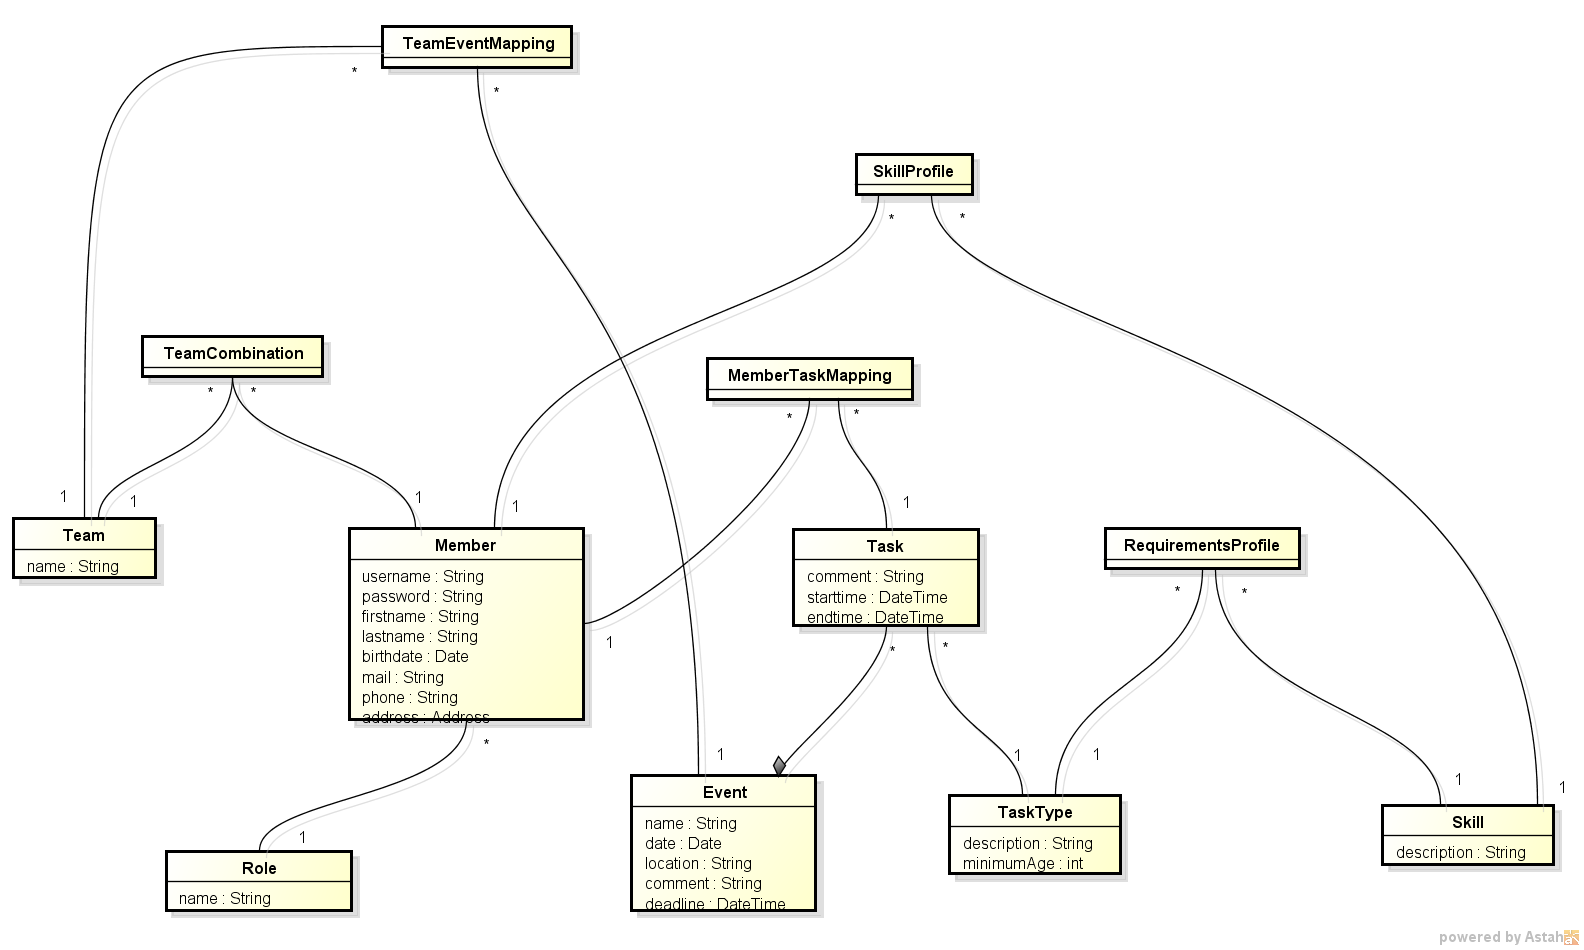
\includegraphics[width=0.9\textwidth]{content/domainanalyse/images/Datamodell.png}
		    \caption{Data Model}
		\end{figure}
    \chapter{Systemsequenzdiagramm}
    \chapter{Systemoperationen}
	

    % \chapter{Playground}
\section{A Playground section}        

\subsection{hoi test SUBSUB Section}
\subsubsection{hoi test SUBSUB Section}
Lorem ipsum dolor sit amet, consectetuer adipiscing elit. Aenean commodo ligula eget dolor. Aenean massa. Cum sociis natoque penatibus et magnis dis parturient montes, nascetur ridiculus mus. Donec quam felis, ultricies nec, pellentesque eu, pretium quis, sem. Nulla consequat massa quis enim. Donec pede justo, fringilla vel, aliquet nec, vulputate eget, arcu.

In enim justo, rhoncus ut, imperdiet a, venenatis vitae, justo. Nullam dictum felis eu pede mollis pretium. Integer tincidunt. Cras dapibus. Vivamus elementum semper nisi. Aenean vulputate eleifend tellus. Aenean leo ligula, porttitor eu, consequat vitae, eleifend ac, enim. Aliquam lorem ante, dapibus in, viverra quis, feugiat a, tellus.

Phasellus viverra nulla ut metus varius laoreet. Quisque rutrum. Aenean imperdiet. Etiam ultricies nisi vel augue. Curabitur ullamcorper ultricies nisi. Nam eget dui. Etiam rhoncus. Maecenas tempus, tellus eget condimentum rhoncus, sem quam semper libero, sit amet adipiscing sem neque sed ipsum. Nam quam nunc, blandit vel, luctus pulvinar, hendrerit id, lorem. Maecenas nec odio et ante tincidunt tempus. Donec vitae sapien ut libero venenatis faucibus. Nullam quis ante. Etiam sit amet orci eget eros faucibus tincidunt. Duis leo. Sed fringilla mauris sit amet nibh. Donec sodales sagittis magna. Sed consequat, leo eget bibendum sodales, augue velit cursus nunc,

\section{Code Listings}
\begin{lstlisting}[language=CSharp, caption=Hello World in C\#, label=lst:helloWorldCSharp, firstnumber=1]
// A Hello World! program in C#.
using System;
namespace HelloWorld
{
    class Hello 
    {
        static void Main() 
        {
            Console.WriteLine("Hello World!");

            // Keep the console window open in debug mode.
            Console.WriteLine("Press any key to exit.");
            Console.ReadKey();
        }
    }
}
\end{lstlisting}

\begin{lstlisting}[language=JavaScript, caption=JavaScript Hello Wordl, label=lst:helloWorldJavaScript, firstnumber=1]
//Ausgabe von Hallo Welt! mit einer Alert-Box
alert("Hallo Welt!");
\end{lstlisting}

\section{Text}
Eine ``Beispiel'' Auflistung
\begin{itemize}
    \item Item mit \emph{krusivem} Text
    \item Item mit \textbf{fettem} Text
\end{itemize}

\subsection{Bild}
\begin{figure}[ht]
    
\includegraphics[height=5cm]{template/images/hsrlogo.png}
    \caption{HSR Logo}
\end{figure}


\chapter{Tables}
\section{Meilensteine}

\begin{table}[H]
    \tablestyle
    \tablealtcolored
    \begin{tabularx}{\textwidth}{l l l X}
        \tableheadcolor
            \tablehead ID &
            \tablehead Meilenstein &
            \tablehead Termin &
            \tablehead Beschreibung \tabularnewline
        \tablebody
            \textit{M1}\label{M1} & Ende Inception & 07.03.2014
                & bla bla bla \tabularnewline
            \textit{M2} & Ende Elaboration & 17.03.2014
                & Bla bla bla \tabularnewline
            \textit{..} & .. & ..
                & .. \tabularnewline
            \textit{..} & .. & ..
                & .. \tabularnewline
        \tableend
    \end{tabularx}
    \caption{Meilensteine}
\end{table}

\begin{table}[H]
    \tablestyle
    \tablealtcolored
    \begin{tabularx}{\textwidth}{l X l}
        \tableheadcolor
            \tablehead Topic &
            \tablehead Erläuterung \tabularnewline
        \tablebody
        \textit{Lorem 1} &
            Lorem ipsum dolor sit amet, consectetuer adipiscing elit. Aenean commodo ligula eget dolor. Aenean massa. Cum sociis natoque penatibus et magnis dis parturient montes, nascetur ridiculus mus. Donec quam felis, ultricies nec, pellentesque eu, pretium quis, sem. Nulla consequat massa quis enim. Donec pede justo, fringilla vel, aliquet nec, vulputate eget, arcu.
            \tabularnewline
        \textit{Lorem 2} &
            In enim justo, rhoncus ut, imperdiet a, venenatis vitae, justo. Nullam dictum felis eu pede mollis pretium. Integer tincidunt. Cras dapibus. Vivamus elementum semper nisi. Aenean vulputate eleifend tellus. Aenean leo ligula, porttitor eu, consequat vitae, eleifend ac, enim. Aliquam lorem ante, dapibus in, viverra quis, feugiat a, tellus.
            \tabularnewline
        \textit{Lorem 3} &
            Phasellus viverra nulla ut metus varius laoreet. Quisque rutrum. Aenean imperdiet. Etiam ultricies nisi vel augue. Curabitur ullamcorper ultricies nisi. Nam eget dui. Etiam rhoncus. Maecenas tempus, tellus eget condimentum rhoncus, sem quam semper libero, sit amet adipiscing sem neque sed ipsum. Nam quam nunc, blandit vel, luctus pulvinar, hendrerit id, lorem. Maecenas nec odio et ante tincidunt tempus. Donec vitae sapien ut libero venenatis faucibus. Nullam quis ante. Etiam sit amet orci eget eros faucibus tincidunt. Duis leo. Sed fringilla mauris sit amet nibh. Donec sodales sagittis magna. Sed consequat, leo eget bibendum sodales, augue velit cursus nunc,
            \tabularnewline
        \tableend
    \end{tabularx}
    \caption{Topic Listing}
\end{table}

\begin{table}[H]
    \newcolumntype{s}{>{\centering\hsize=0.15\hsize}X}
    \tablestyle
    \tablealtcolored
    \begin{tabularx}{\textwidth}{X s s s s s s s}
        \tableheadcolor
            \tablehead &
            \rotatebox{90}{\bfseries\textit{TK1 Eigenkonzepte} } &
            \rotatebox{90}{\bfseries\textit{TK2 Eignung}} &
            \rotatebox{90}{\bfseries\textit{TK3 Produktreife}} &
            \rotatebox{90}{\bfseries\textit{TK4 Aktualität}} &
            \rotatebox{90}{\bfseries\textit{TK5 ``Ease of use''}} &
            \rotatebox{90}{\bfseries\textit{TK6 Testbarkeit}} &
            \rotatebox{90}{\bfseries\textit{Gesamtbewertung}}
            \tabularnewline
        \tablebody
            \textit{Ruby on Rails} &
            \oneStar &
            \oneStar &
            \threeStars &
            \oneStar &
            \threeStars &
            \twoStars &
            4
            \tabularnewline
        \tableend
    \end{tabularx}
    \caption{Bewertung Ruby on Rails}
\end{table}

\begin{figure}[H]
    \begin{table}[H]
        \tablestyle
        \tablealtcolored
        \begin{tabularx}{\textwidth}{l c c X}
            \tableheadcolor
                \tablehead Richtlinie &
                \tablehead\rotatebox{90}{Nutzen} &
                \tablehead\rotatebox{90}{Demonstriert\hspace{3mm}} &
                \tablehead Bemerkung
                \tabularnewline
            \tablebody
                Richtline 1 & \faSmile & \faOk & Wiederverwendbare API umgesetzt\tabularnewline
                Richtline 2 & \faSmile & \faOk & Facebook als Identity-Provider\tabularnewline
                Richtline 3 & \faMeh & \faOk & \tabularnewline
                Richtline 4 & \faSmile & \faOk & Make\tabularnewline
            \tableend
        \end{tabularx}
    \end{table}
    \caption{Übersicht Architekturrichtlinienanalyse (2/2)}
    \label{tab:overview-principle-demonstration-2}
\end{figure}

\begin{figure}[H]
    \begin{table}[H]
        \tablestyle
        \tablealtcolored
        \begin{tabularx}{\textwidth}{X | c c c c c | c c c c | c c}
            \tableheadcolor
                \tablehead &
                \multicolumn{5}{c|}{\bfseries\textit{Backend}} &
                \multicolumn{4}{c|}{\bfseries\textit{Frontend}} &
                \bfseries\textit{Tools}
                \tabularnewline
            \tableheadcolor
                \tablehead &
                \rotatebox{90}{Models} &
                \rotatebox{90}{Businesslogik} &
                \rotatebox{90}{Autentifizierung} &
                \rotatebox{90}{Rendering Engine} &
                \rotatebox{90}{Service Interface} &
                \rotatebox{90}{HTML Markup} &
                \rotatebox{90}{CSS Styling} &
                \rotatebox{90}{JavaScript Code} &
                \rotatebox{90}{Struktur} &
                \xspace
                \tabularnewline
            \tablebody
                RP1 REST & & & & & \faOk & & & & & \tabularnewline
                RP2 Application logic & & \faOk & & & & & & & & \tabularnewline
                RP3 HTTP & & & & & \faOk & & & & & \tabularnewline
                RP4 Link & & & & & \faOk & & & & \faOk & \tabularnewline
                RP5 Non-Browser & & & & & \faOk & & & & & \tabularnewline
                RP6 Should-Formats & & & & & \faOk & & & & & \tabularnewline
                RP7 Auth & & & \faOk & & & & & & & \tabularnewline
                RP8 Cookies & & & \faOk & & \faOk & & & & & \tabularnewline
                RP9 Session & & & \faOk & & & & & & \faOk & \tabularnewline
                RP10 Browser-Controls & & & & \faOk & & & & \faOk & \faOk & \tabularnewline
                RP11 POSH & & & & \faOk & & \faOk & \faOk & & & \tabularnewline
                RP12 Accessibility & & & & \faOk & & \faOk & \faOk & & & \tabularnewline
                RP13 Progressive Enhancement & & & & & & \faOk & \faOk & \faOk & & \tabularnewline
                RP14 Unobtrusive JavaScript & & & & & & \faOk & & \faOk & & \tabularnewline
                RP15 No Duplication & \faOk & \faOk & & \faOk & &  \faOk &  \faOk & \faOk & & \tabularnewline
                RP16 Know Structure & & & & & \faOk & \faOk & \faOk & & & \tabularnewline
                RP17 Static Assets & & & & & & & \faOk & \faOk & & \faOk \tabularnewline
                RP18 History API & & & & & & & & \faOk & & \tabularnewline
                TP3 Eat your own API dog food & & & & & \faOk & & & & & \tabularnewline
                TP4 Separate user identity and sign-up (...) & & & \faOk & & & & & & & \tabularnewline
                TP7 Apply the Web instead of working around & & & & & \faOk & \faOk & \faOk & \faOk & \faOk & \tabularnewline
                TP8 Automate everything or you will be hurt & & & & & & & & & & \faOk \tabularnewline
            \tableend
        \end{tabularx}
    \end{table}
    \caption{Mapping Architekturrichtlinien - Systemkomponenten}
    \label{fig:how-to-show-principles-matrix}
\end{figure}


\chapter{New Page}
\newpage
\section{New Paged}

    
    
\end{document}
